\section{Random Numbers}

All the functions for this task are implemented in random\_numbers.py.
The file random\_walk.py executes the code.

\subsection{Linear Congruental Gemerator (LCG)}

The first exercise was to implement the LCG.
In order to do this the LCG must be initialized with an overall value Xlcg.

\listfile{../src/random_numbers.py}{src/random\_numbers.py}{5}{9}{Initialization of LCG}{initlcg}

The next step is to perform the LCG; therefore a function LCG() is implemented in code block \ref{lcg}.
As you can see the values m, a and c are already given as optional parameters.

\listfile{../src/random_numbers.py}{src/random\_numbers.py}{11}{17}{LCG}{lcg}

Later we want to use the time.time() as a starting value. 
Therefore the function do2int() is defined which converts a float into an integer by passing the decimal marker after the last relevant number.

\listfile{../src/random_numbers.py}{src/random\_numbers.py}{25}{32}{do2int}{do2int}

At last the function normal\_LCG() returns a normalized value in [0,1].
Therefore the result must be divided by m-1.\\

Now it is time to run the random number generator and simulate a random walk. 
Therefor the function random\_walk() is used to generate an 1D random walk with a maximum velocity of $\pm 0.5$ per time step.

\listfile{../src/random_numbers.py}{src/random\_numbers.py}{34}{47}{Random walk}{walk}

The script random\_walk.py takes an optional command line parameter --Xlcg. 
You can use it to set the starting value Xlcg manually.
If it is not given do2int(time.time()) is used.
Notice, that you have to use python3 in order to get good results from the time function.\\

If you perform the random walk several times with the same --Xlcg the trajectory appears to be the same every time. 
By using time.time() as initialization you obey completely different trajectories every time. 
You can see one of this trajectories in graphic \ref{randwalk}.

\begin{figure}[ht]
	\centering
	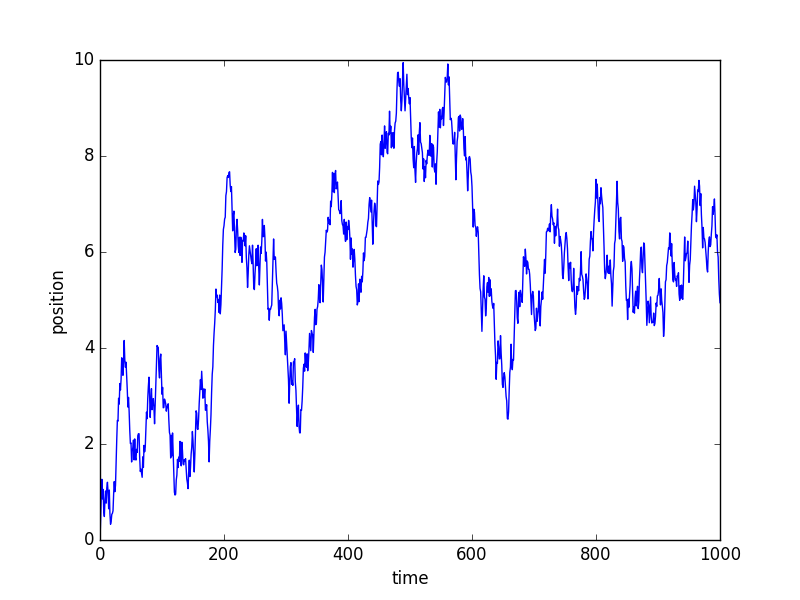
\includegraphics[width=0.7\textwidth]{../dat/random_walk.png}
	\caption{
		Random walk for initialization with time.time().
		}
	\label{randwalk}
\end{figure}

To conclude, the LCG is not really a good random number generator.
Although it takes a long time until the numbers repeat in the same order in between, there can be no number which was already obeyed.
Due to this the random numbers are correlated especially for many used numbers.
Furthermore a bad choice of m, a and c will lead to very bad and no longer uniform random number distribution.

\FloatBarrier

\subsection{Box-Muller (BM)}

The next exercise is to transform uniformly distributed random numbers into 
normal distributed one. 
Therefor the Box-Muller transform is given.
It's implementation is split up into two functions.
calc\_BM() takes two uniform distributed random numbers u1 and u2 and returns the function from the worksheet. 
The function BM() arranges the usage of calc\_BM() in a way that allows to obey an array of $N>1$ normal distributed random numbers. 
In order to get better results the function random.random() which returns better uniformly distributed random numbers is used instead of LCG().

\listfile{../src/random_numbers.py}{src/random\_numbers.py}{51}{65}{Box-Muller}{bm}

The function gauss() just returns the Gaussian probability distribution:
\begin{align}
p(x) 
	&= \frac{1}{\sqrt{2\pi}\sigma}\dot{\Exp{-\frac{x^2}{2\sigma^2}}}
	\label{gauss}
\end{align}

Analogous the function gauss\_3d() returns the three dimensional Gaussian:
\begin{align}
p(\ovec{r}) 
&= \sqrt{\frac{2}{\pi}}\frac{\ovec{r}^2}{\sigma^3}\dot{\Exp{-\frac{\ovec{r}^2}{2\sigma^2}}}
\label{gauss3d}
\end{align}

In order to test the BM a function show\_BM\_hist() was created.
It draws a histogram of 1000 by the BM() created random numbers in a diagram with the gauss().
You can pass different $\sigma$, $\mu$ and therefor also new x-axis-limits.
The option bars states how many bars you want to have for the histogram.
The results can be seen in graphic \ref{bmhist}.

\listfile{../src/random_numbers.py}{src/random\_numbers.py}{73}{88}{Box-Muller histogram}{showbmhist}

\begin{figure}[ht]
	\centering
	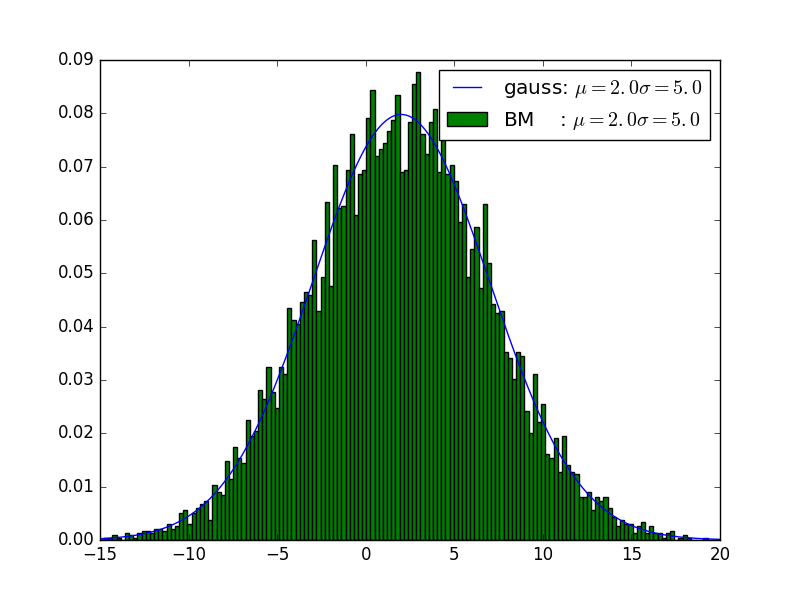
\includegraphics[width=0.7\textwidth]{../dat/BM_hist.png}
	\caption{
		Histogram of the BM random number distribution and the Gaussian function \eqref{gauss}.
	}
	\label{bmhist}
\end{figure}

The last exercise was to transform the same principal into three dimensions.
You can use the function rand\_vel\_vec() in order to create a $N\times 3$ vector of BM random numbers (velocity vector). 
The function show\_vel\_hist() in code block \ref{showvelhist} takes the absolute values of this velocities vel\_abs and draws them as histogram against the three dimensional Gaussian \eqref{gauss3d}.

\listfile{../src/random_numbers.py}{src/random\_numbers.py}{105}{120}{3D Box-Muller histogram}{showvelhist}

\begin{figure}[ht]
	\centering
	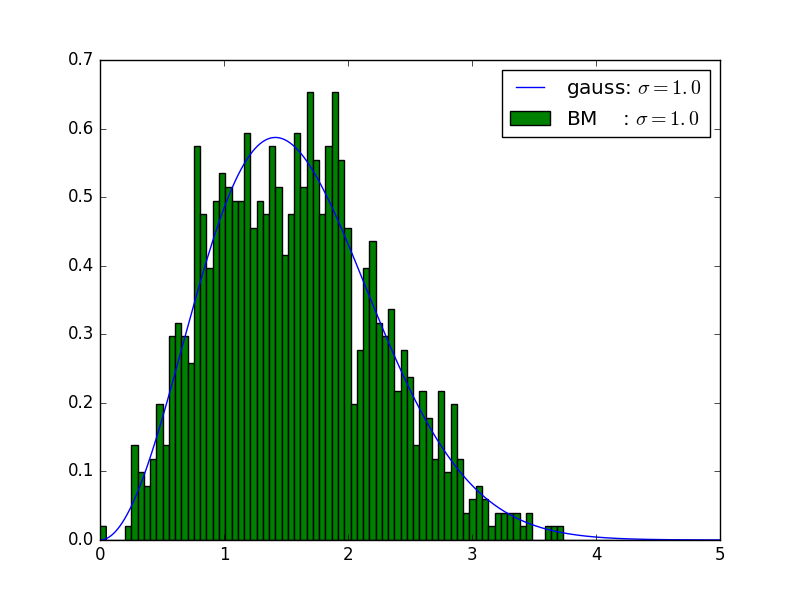
\includegraphics[width=0.7\textwidth]{../dat/vel_hist.png}
	\caption{
		Histogram of the BM random velocities and the 3D Gaussian function \eqref{gauss3d}.
	}
	\label{velhist}
\end{figure}

As you can see the histograms fit to the expected distribution in both cases.\\

Notice that it would not make sense to set an $\mu\neq 0$ unless you have a drift which means an overall velocity trend in a specific direction. 

\FloatBarrier